\chapter{istar: software as a service}

\section{Abstract}

Protein-ligand docking is a key computational method in the design of starting points for the drug discovery process. Performing large-scale docking requires tedious configurations of necessary tools and preparations of mandatory materials. Although a few online docking platforms exist, they neither support fine-grained ligand selection based on molecular properties and previewing the number of ligands to dock, nor be able to monitor job progress in real time. They also lack convenient visualization of docking results and straightforward output of compound suppliers.

We are motivated by the desire to automate large-scale docking using our popular docking engine idock and thus have developed a publicly accessible web platform called istar. Without cumbersome software installation, users can submit jobs using our website. Our istar website supports 1) filtering ligands by desired molecular properties and previewing the number of ligands to dock, 2) monitoring job progress in real time, and 3) visualizing ligand conformations and outputting free energy predicted by idock, binding affinity predicted by RF-Score, putative hydrogen bonds, and supplier information for easy purchasing, three useful features commonly lacked on other online docking platforms like DOCK Blaster or iScreen. We have collected 23,129,083 ligands from the All Clean subset of the ZINC database, and revamped our idock to version 2.0, further improving docking speed and accuracy, and integrating RF-Score as an alternative rescoring function.

To compare idock 2.0 with the state-of-the-art AutoDock Vina 1.1.2, we carried out a rescoring benchmark and a redocking benchmark on the 2,897 and 343 protein-ligand complexes of PDBbind v2012 refined set and CSAR NRC HiQ Set 24Sept2010 respectively, and an execution time benchmark on 12 diverse proteins and 3,000 ligands of different molecular weight. Results showed that, under various scenarios, idock achieved comparable success rates while outperforming AutoDock Vina in terms of docking speed by at least 8.69 times and at most 37.51 times. When evaluated on the PDBbind v2012 core set, our istar platform in combination with RF-Score managed to reproduce Pearson and Spearman correlation coefficients of as high as 0.855 and 0.859, respectively, between the experimental binding affinity and the predicted binding affinity of the docked conformation. istar::idock is freely available at http://istar.cse.cuhk.edu.hk/idock.

This was a collaborative project with Pedro J. Ballester from European Bioinformatics Institute, Cambridge, United Kingdom. It was published in \textit{PLoS ONE} on 24 January 2014 \citep{1362}.

%Shiv Gupta, using literature search for the project I came through istar a wonderful platform for protein-ligand interaction prediction.

\section{Introduction}

Protein-ligand docking predicts the preferred conformation and binding affinity of a small ligand as non-covalently bound to the specific binding site of a protein. Docking can therefore be used not only to determine whether a ligand binds, but also to understand how it binds. The latter is subsequently important to improve the potency and selectivity of binding. To date, there are hundreds of docking tools \citep{493,922}. The AutoDock series \citep{597,596,595} is the most cited docking software in the research community, with over 9,400 citations according to Google Scholar. AutoDock contributed to the discovery of several drugs, including the first clinically approved inhibitor of HIV integrase \citep{1169}. Following its initial release, several parallel implementations were developed using either multithreading or computer cluster \citep{115,560,782}.

In 2009, AutoDock Vina \citep{595} was released. As the successor of AutoDock 4 \citep{596}, AutoDock Vina significantly improves the average accuracy of the binding mode predictions while running two orders of magnitude faster with multithreading \citep{595}. It was compared to AutoDock 4 on selecting active compounds against HIV protease, and was recommended for docking large molecules \citep{556}. Its functionality of semi-flexible protein docking by enabling flexibility of side-chain residues was evaluated on VEGFR-2 \citep{1084}. To further facilitate the usage of AutoDock Vina, auxiliary tools were subsequently developed, including a PyMOL (http://www.pymol.org) plugin for program settings and visualization \citep{609}, a bootable operating system for computer clusters \citep{773}, a console application for virtual screening on Windows \citep{1268}, and a GUI for virtual screening on Windows \citep{1250}.

In 2011, inspired by AutoDock Vina, we developed idock 1.0 \citep{1153}, a multithreaded virtual screening tool for flexible ligand docking. idock introduces plenty of innovations, such as caching receptor and grid maps in memory to permit efficient large-scale docking, revised numerical model for much faster energy approximation, and capability of automatic detection of inactive torsions for dimensionality reduction. When benchmarked on docking 10,928 drug-like ligands against HIV reverse transcriptase, idock 1.0 achieved a speedup of 3.3 in terms of CPU time and a speedup of 7.5 in terms of elapsed time on average compared to AutoDock Vina, making idock one of the fastest docking software.

Having released idock, we kept receiving docking requests from our colleagues and collaborators. They are mostly biochemists and pharmacologists, outsourcing the docking research to us after discovering pharmaceutical protein targets for certain diseases of therapeutic interest. Consequently, we had to grab the protein structure, do format conversion, define search space, set up docking parameters, and keep running idock in batch for months. Tedious enough, all the above work was done manually, resulting in very low research productivity. In order to automate large-scale protein-ligand docking using our idock, we have therefore developed a web platform called istar.

A few online docking platforms already exist. DOCK Blaster \citep{557} investigates the feasibility of full automation of protein-ligand docking. It utilizes DOCK 3 \citep{1445} as the docking engine and ZINC \citep{532,1178} as the ligand database. It also utilizes PocketPickker (CLIPPERS) \citep{395} for binding pocket identification. iScreen \citep{899} is a compacted web server for TCM (Traditional Chinese Medicine) docking and followed by customized \textit{de novo} drug design. It utilizes PLANTS \citep{610,607,779} as the docking engine and TCM@Taiwan \citep{528} as the ligand database. It also utilizes LEA3D \citep{1223} for \textit{de novo} ligand design. SwissDock \citep{1425} is a web server dedicated to the docking of small molecules on target proteins. It utilizes EADock DSS \citep{606,781} as the docking engine. FORECASTER \citep{1012} is a web interface consisting of a set of tools for the virtual screening of small molecules binding to biomacromolecules (proteins, receptors, and nucleic acids). It utilizes the flexible-target docking program FITTED \citep{602} as the docking engine. Other web servers for docking include e-LEA3D (http://chemoinfo.ipmc.cnrs.fr/), Sanjeevini (http://www.scfbio-iitd.res.in/sanjeevini/sanjeevini.jsp), DockingServer (http://www.dockingserver.com/web), DockingAtUTMB (http://docking.utmb.edu/), Pardock (http://www.scfbio-iitd.res.in/dock/pardock.jsp), PatchDock (http://bioinfo3d.cs.tau.ac.il/PatchDock/), MetaDock (http://dock.bioinfo.pl/), PPDock (http://140.112.135.49/ppdock/index.html) and MEDock (http://medock.ee.ncku.edu.tw/). A comprehensive list is being kept up to date on the click2drug web portal http://www.click2drug.org/.%\textit{i}Drug \citep{1396} is a web-accessible and interactive drug discovery and design platform. The web interface enables binding sites detection, virtual screening hits identification, and drug targets prediction in an interactive manner through a seamless interface to all adapted packages. Several commercially available compound databases for hit identification and a well-annotated pharmacophore database for drug targets prediction were integrated as well. The web interface provides Java-based tools for real-time molecular building/editing, converting, displaying, and analyzing.

Nevertheless, the above platforms neither support fine-grained ligand selection based on molecular properties and previewing the number of ligands to dock, nor be able to monitor job progress in real time. They lack straightforward output of compound suppliers, a hurdle preventing users from purchasing high-rank compounds for further wet-lab verification. They also lack convenient and interactive online visualization of the docking results. We aim to address these obstacles on our istar platform. Moreover, we strongly emphasize docking efficiency, which we believe is the most crucial factor for public large-scale docking platforms, so we try every endeavor to optimize our docking engine idock. Furthermore, we adopt the robust RF-Score \citep{564} version 3 as a rescoring function for accurate prediction of binding affinity.

Overall, we intend to design istar as a versatile SaaS (Software as a Service) web platform rather than a conventional web server merely for docking purpose. SaaS is part of the nomenclature of cloud computing. It is a software delivery model in which software and associated data are centrally hosted on the cloud, typically accessed by users using a thin client via a web browser. We opt to abstract our software into easy-to-use services to promote their usage by a wide variety of users from different disciplines. In addition to idock for prospective structure-based virtual screening, we have also hosted on istar several other services, for examples, USR (Ultrafast Shape Recognition) \citep{1379} and USRCAT (USR with Credo Atom Types) \citep{1331} for prospective ligand-based virtual screening, iview \citep{1366} for interactive WebGL visualization of protein-ligand complex, igrep \citep{1138} for approximate nucleotide sequence matching, and icuda as an introductory seminar series on CUDA programming.

\section{Methods and materials}

In the following subsections, we introduce our fast docking engine idock, our accurate rescoring function RF-Score, our modern web platform istar, and the experimental settings regarding datasets and benchmarks.

\subsection{Docking engine idock}

The input to idock includes a rigid receptor, a set of flexible ligands, and a cubic box, which is used to restrict the conformational space to a particular binding site of the receptor. The output from idock includes predicted conformations and their predicted binding affinity.

idock consists of two core components, a scoring function to predict binding affinity, and an optimization algorithm to explore the conformational space. idock inherits the same scoring function from AutoDock Vina. The idock score is made up of a conformation-dependent part and a conformation-independent part. The conformation-dependent part is a weighted sum of five terms over all the pairs of atoms $i$ and $j$ that can move relative to each other, excluding 1-4 interactions, i.e. atoms separated by up to three consecutive covalent bonds. The sum is calculated from equations \eqref{istar:e} and \eqref{istar:e_ij} where $t_i$ and $t_j$ are the atom types of $i$ and $j$ respectively, and $r_{ij}$ is their interatomic distance with a cutoff at $r_{ij}$ = 8\AA. The five terms are calculated from equations \eqref{istar:Gauss1} to \eqref{istar:HBonding} where $d_{ij}$ is the surface distance calculated from equation \eqref{istar:d_ij} where $R_{t_i}$ and $R_{t_j}$ are the Van der Waals radii of $t_i$ and $t_j$ respectively. All terms are in \AA\ units. The first three terms account for steric interactions, the fourth term accounts for hydrophobic effect, and the fifth term accounts for hydrogen bonding. Metal ions are treated as hydrogen bond donors. The weighting coefficients are derived from linear regression on the PDBbind \citep{529,530} v2007 refined set ($N$ = 1,300). The optimization algorithm attempts to find the global minimum of $e$ and other low-scoring conformations, which it then ranks.

\begin{equation}
\label{istar:e}
e = \sum_{i < j} e_{ij}
\end{equation}

\begin{eqnarray}
\label{istar:e_ij}
e_{ij} &=& (-0.035579) \times Gauss_1(t_i, t_j, r_{ij}) \nonumber \\
       &+& (-0.005156) \times Gauss_2(t_i, t_j, r_{ij}) \nonumber \\
       &+& (+0.840245) \times Repulsion(t_i, t_j, r_{ij}) \nonumber \\
       &+& (-0.035069) \times Hydrophobic(t_i, t_j, r_{ij}) \nonumber \\
       &+& (-0.587439) \times HBonding(t_i, t_j, r_{ij})
\end{eqnarray}

\begin{equation}
\label{istar:Gauss1}
Gauss_1(t_i, t_j, r_{ij}) = e^{-(d_{ij} / 0.5)^2}
\end{equation}

\begin{equation}
\label{istar:Gauss2}
Gauss_2(t_i, t_j, r_{ij}) = e^{-((d_{ij} - 3) / 2)^2}
\end{equation}

\begin{equation}
\label{istar:Repulsion}
Repulsion(t_i, t_j, r_{ij}) =
\begin{cases}
d_{ij}^2 & \text{if } d_{ij} < 0\\
0 &\text{if } d_{ij} \geq 0
\end{cases}
\end{equation}

\begin{equation}
\label{istar:Hydrophobic}
Hydrophobic(t_i, t_j, r_{ij}) =
\begin{cases}
1 & \text{if } d_{ij} \leq 0.5\\
1.5 - d_{ij} & \text{if } 0.5 < d_{ij} < 1.5\\
0 & \text{if } d_{ij} \geq 1.5\\
\end{cases}
\end{equation}

\begin{equation}
\label{istar:HBonding}
HBonding(t_i, t_j, r_{ij}) =
\begin{cases}
1 & \text{if } d_{ij} \leq -0.7\\
d_{ij} / (-0.7) & \text{if } -0.7 < d_{ij} < 0\\
0 & \text{if } d_{ij} \geq 0\\
\end{cases}
\end{equation}

\begin{equation}
\label{istar:d_ij}
d_{ij} = r_{ij} - (R_{t_i} + R_{t_j})
\end{equation}

The conformation-dependent part can be seen as the sum of inter-molecular and intra-molecular contributions. Hence equation \eqref{istar:e} can be rewritten into equation \eqref{istar:inter+intra} where $e_{inter}$ is the summation over all the heavy atom pairs between the receptor and the ligand, and $e_{intra}$ is the summation over all the non 1-4 heavy atom pairs of the ligand.

\begin{equation}
\label{istar:inter+intra}
e = e_{inter} + e_{intra}
\end{equation}

The conformation-independent part penalizes $e_{inter}$ for ligand flexibility. The predicted free energy of the $k$th conformation for output, denoted as $e'_k$, is calculated from equation \eqref{istar:FlexibilityPenalty} where $k$ is the subscript for conformation, $e_k$ is the conformation-dependent score of the $k$th conformation calculated from equation \eqref{istar:e}, $e_{intra,1}$ is the $e_{intra}$ of the first, i.e. lowest-scoring conformation, $N_{ActiveTors}$ is the number of active torsions and $N_{InactiveTors}$ is the number of inactive torsions of the ligand. A torsion is called inactive in this context if its arbitrary values do not affect the overall output of the scoring function. Note that $e_{intra,1}$, rather than $e_{intra,k}$, is subtracted in order to preserve the ranking of predicted conformations.

\begin{equation}
\label{istar:FlexibilityPenalty}
e'_k = \frac{e_k - e_{intra,1}}{1 + 0.05846 \times (N_{ActiveTors} + 0.5 \times N_{InactiveTors})}
\end{equation}

On one hand, in order to fast evaluate $e_{ij}$, idock precalculates some of its possible values. Note from equation \eqref{istar:e_ij} that $e_{ij}$ is essentially a function of three variables, namely $t_i$, $t_j$, and $r_{ij}$, which all have known lower and upper bounds. There are 15 heavy atom types implemented in idock, so there are 15*16/2=120 different combinations of pairs of $t_i$ and $t_j$. Since $r_{ij}$ is cut off at 8\AA, idock uniformly samples 65,536 $r_{ij}$ values in the range [0, 8] and precalculates their $e_{ij}$ values. Subsequently in building grid maps or calculating $e_{intra}$, given a combination of $t_i$, $t_j$ and $r_{ij}$, idock approximates the true value of $e_{ij}$ simply by a table lookup, rather than by a table lookup followed by a linear interpolation in the case of AutoDock Vina.

On the other hand, in order to fast evaluate $e_{inter}$, idock precalculates its possible values by building grid maps. A grid map of atom type \textit{t} is constructed by placing virtual probe atoms of atom type \textit{t} along the X, Y, Z dimensions of the search box at a certain granularity. The $e_{inter}$ value of these probe atoms are precalculated from equation \eqref{istar:e_ij}. Subsequently in the conformational optimization stage, given a sampled conformation, idock approximates the true values of $e_{inter}$ of ligand heavy atoms simply by a table lookup rather than by a table lookup followed by a linear interpolation in the case of AutoDock Vina. In fact, when we profiled AutoDock Vina, its linear interpolation of the 8 nearest corner probe atoms turned out to be a performance bottleneck because it involves 8 readings, 12 subtractions, 24 multiplications, and 7 additions. The grid granularity is hard-coded to be a coarse value of 0.375\AA\ in AutoDock Vina, while in idock it is exposed as a program option for users to adjust accordingly and has a default fine value of 0.15625\AA\ so as to complement the possible precision loss due to the removal of linear interpolation for the sake of performance.

Likewise in AutoDock Vina, idock also uses Broyden-Fletcher-Goldfarb-Shanno (BFGS) \citep{786}, a quasi-Newton algorithm, for local optimization. In each BFGS iteration, a conformational mutation and a line search are taken, with each sampled conformation being accepted according to the Metropolis criterion. The number of iterations correlates to the complexity of the ligand in terms of the number of heavy atoms and the number of torsions. BFGS approximates the inverse Hessian matrix. In other words, it uses not only the value of the scoring function but also its gradient, which are the derivatives of the scoring function with respect to the position, orientation and torsions of the ligand. Although both programs share similar optimization algorithms, their internal implementations differ substantially. In idock, the BFGS local optimization stops if and only if no appropriate step length can be obtained by line search, thus increasing the probability of finding optimal local minimums. More optimization runs with fewer number of BFGS iterations are executed, better balancing high conformational diversity and short execution time.

idock introduces a novel feature that can automatically detect and deactivate certain torsions which are activated in the input file but indeed have no impact on the overall scoring. These are the torsions of hydroxyl groups \textemdash{OH}, amine groups \textemdash{NH$_2$} and methyl groups \textemdash{CH$_3$}, where mere hydrogens will be rotated and therefore have no contributions to the idock score. idock is capable of re-classifying them as inactive torsions during parsing, thus reducing the dimension of variables to optimize in subsequent BFGS iterations.

idock encapsulates many other improvements. Please refer to its change log for a complete list of new features and bugfixes.

\subsection{Scoring function RF-Score}

RF-Score \citep{564} is a member of a new class of scoring functions that use non-parametric machine learning approach to predict binding affinity in an entirely data-driven manner. It is the first application of RF (Random Forests) \citep{1309} to predicting protein-ligand binding affinity. It was rigorously shown \citep{564} to perform better than 16 classical scoring functions in ranking protein-ligand complexes according to their predicted binding affinity. It was also shown to be useful in the discovery of new molecular scaffolds in antibacterial hit identification \citep{1281}.

In RF-Score, each feature comprises the number of occurrences of a particular protein-ligand atom type pair interacting within a certain distance range. Four common atom types for the protein (C, N, O, S) and nine common atom types for the ligand (C, N, O, F, P, S, Cl, Br, I) constitute a vector of 36 features, and the distance cutoff is chosen to be as sufficiently large as 12\AA\ so as to implicitly capture solvation effects.

RF grows each binary tree without pruning using the CART algorithm \citep{1310} from a bootstrap sample of the training data. It selects the best split at each node of the tree from a typically small number of randomly chosen features, and terminates splitting a node when it contains no more than five samples. The prediction from an individual tree is the arithmetic mean of its sample outputs in the traversed leaf node. The final prediction is the arithmetic mean of the individual predictions of all the trees in the forest. The performance of RF-Score does not vary significantly with the number of trees beyond a certain threshold. The common practice is to use 500 as a sufficiently large number of trees.

The original version of RF-Score \citep{564} was trained on PDBbind v2007 refined set less the core set ($N$ = 1,105). We re-trained RF-Score on PDBbind v2013 refined set ($N$ = 2,959) for prospective prediction purpose, and integrated it into our istar platform to re-score predicted conformations. We also implemented a consensus score as the average effect of idock score and RF-Score. Mathematically, equations \eqref{istar:DeltaG} to \eqref{istar:pKd} relate equilibrium constant $K_{eq}$ and dissociation constant $K_d$ with Gibbs free energy $\Delta G$, where $R$ is gas constant $R = 1.9858775 \times 10^{-3} kcal/mol$ and $T$ is absolute temperature.

\begin{equation}
\label{istar:DeltaG}
\Delta G = -RT\ln K_{eq}
\end{equation}

\begin{equation}
\label{istar:Kd}
K_d = \frac{1}{K_{eq}}
\end{equation}

\begin{equation}
\label{istar:pKd}
pK_d = -\log_{10} K_d
\end{equation}

Assuming $T = 298.15K$ at room temperature, plugging equations \eqref{istar:Kd} and \eqref{istar:pKd} into \eqref{istar:DeltaG} yields

\begin{equation}
\label{istar:pKd=DeltaG}
pK_d = -0.73349480509 \times \Delta G
\end{equation}

Equation \eqref{istar:pKd=DeltaG} transforms the predicted free energy output by idock in $kcal/mol$ into binding affinity in $pK_d$ unit. The consensus score is thus defined in equation \eqref{istar:Consensus} so that it directly reflects the predicted potency in $pK_d$ unit.

\begin{equation}
\label{istar:Consensus}
ConsensusScore = 0.5 \times (-0.73349480509 \times idockScore + RFScore)
\end{equation}

\subsection{Web platform istar}

Figure \ref{istar:Architecture} shows the overall architecture of istar. There are five major components: a website, a web server, a database management system, several workstations, and a network file system. Under typical circumstances, a user browses our website and submits a job. The web server first validates user input and then saves it into the database. Several workstations keep running daemons, which fetch jobs from the database and perform protein-ligand docking. Upon completion, the daemon sends a notification email to the user and writes the results to the network file system, which are cached as static contents by the web server. The user again browses our website to download or visualize the results, or monitor job progress. Our web server also supports REST API for developers to program against. Instructions on how to use the REST API can be found at http://istar.cse.cuhk.edu.hk/idock.

\begin{figure}
\centering
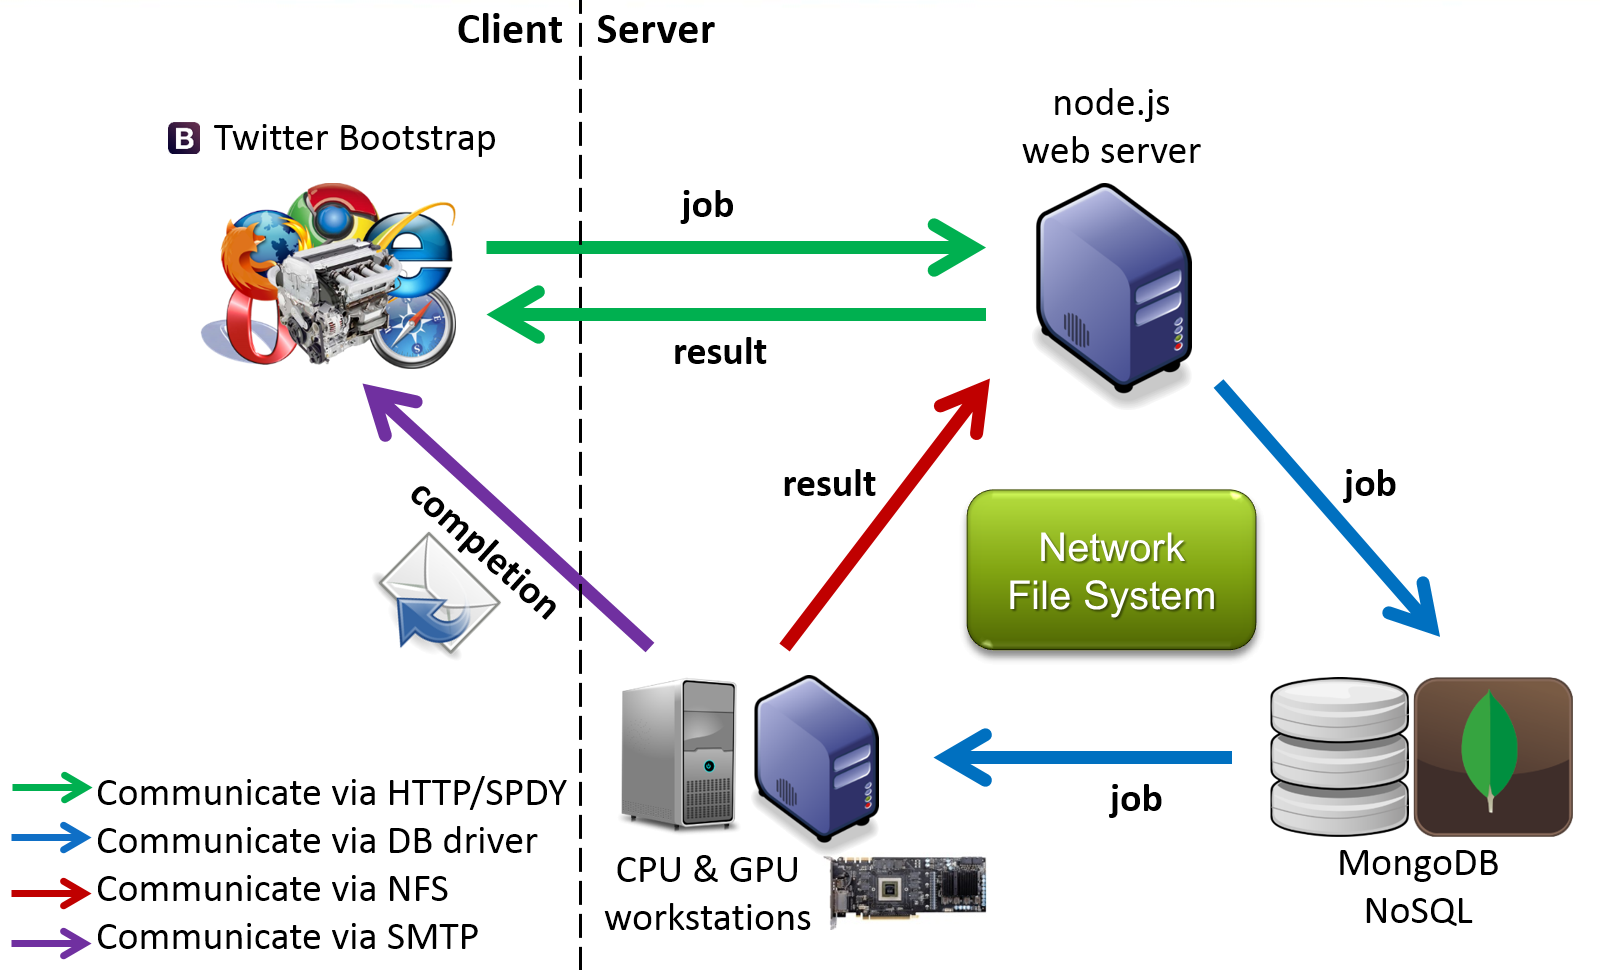
\includegraphics[width=\linewidth]{../istar/Architecture.png}
\caption{istar architecture.}
\label{istar:Architecture}
\end{figure}

In our istar::idock web page (Figure \ref{istar:idock}), the first section displays summary of existing jobs and the second section allows new job submission. A job comprises compulsory fields and optional fields. The compulsory fields include a receptor in PDB format, a search space defined by a cubic box, a brief description about the job, and an email to receive completion notification. The optional fields include nine ligand filtering conditions. The nine ligand filtering conditions are molecular weight, partition coefficient xlogP, apolar desolvation, polar desolvation, number of hydrogen bond donors, number of hydrogen bond acceptors, topological polar surface area tPSA, net charge, and number of rotatable bonds. These nine molecular descriptors were directly retrieved from our data source, i.e. the ZINC database \citep{532,1178}, in which the nine descriptors were already precalculated. Note that although molecular mass in Dalton unit might be a more appropriate descriptor than molecular weight in g/mol unit, we stick to the latter in order to maintain consistency with ZINC, in which the g/mol unit is used for molecular weight.

\begin{figure}
\centering
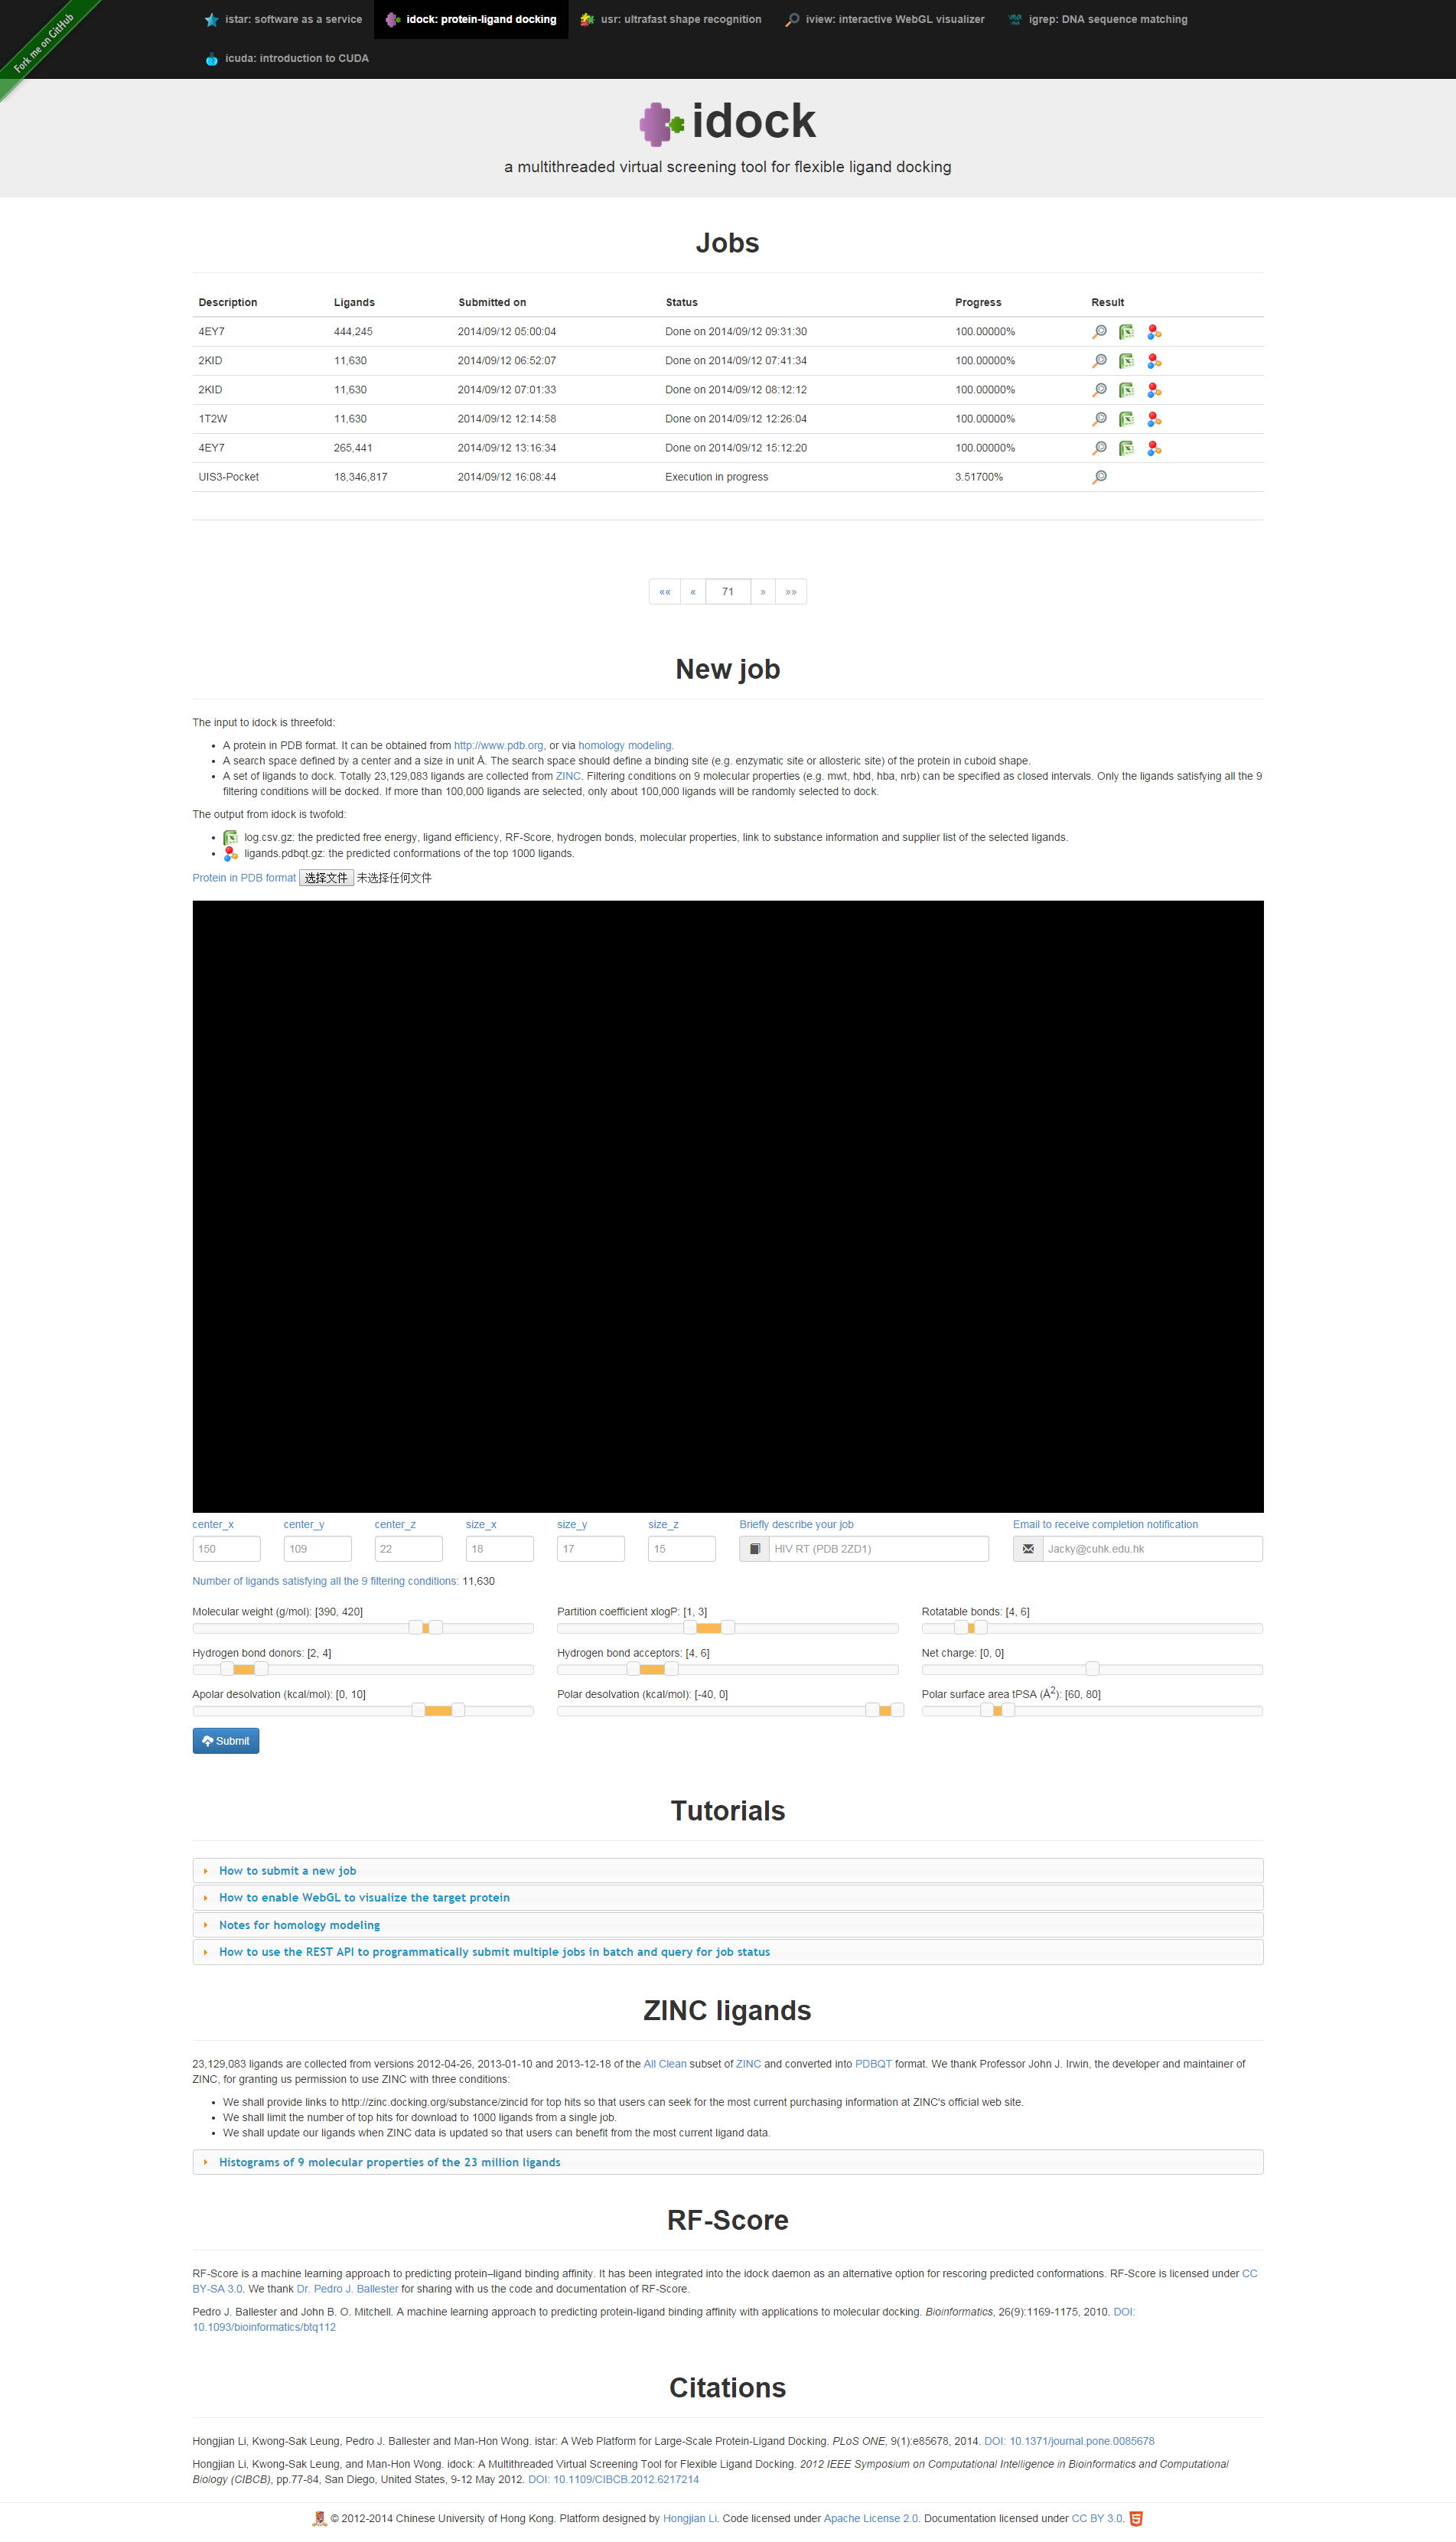
\includegraphics[width=\linewidth]{../istar/idock.png}
\caption{istar::idock web page.}
\label{istar:idock}
\end{figure}

We collected 23,129,083 ligands at pH 7 in mol2 format from versions 2012-04-26, 2013-01-10 and 2013-12-18 of the All Clean subset the ZINC database \citep{532,1178} with explicit permission from its major developer and maintainer. The All Clean subset was constituted by applying the strict filtering rules specified at http://blaster.docking.org/filtering, e.g. aldehydes and thiols were removed. We then converted the entire database of ligands in batch into PDBQT format as used by idock. The huge number of 23 million ligands should be sufficient for most prospective applications. In case users need to screen their own ligand libraries, at present we recommend running idock locally on their computers.

istar supports ligand selection by desired molecular properties in a fine-grained manner and previewing the number of ligands to dock in real time (Figure \ref{istar:idock}, middle section). Users can move the nine sliders to filter ligands in the form of closed intervals. Only the ligands satisfying all the nine filtering conditions will be docked. Because of the relationship of logical and, in order to nullify a specific filtering condition, one may expand its closed interval to cover the entire possible range. We set up default values of the lower and upper bounds of the nine molecular properties for novices to get started quickly.

istar supports monitoring job progress in real time (Figure \ref{istar:idock}, top section). We composed a timer to regularly poll the server and automatically fetch and report the latest job progress every second without page refresh. Users can thus have a rough estimation in advance of how long the jobs will take and when the jobs will complete. This feature is particularly handy when the jobs are long running, which is usually the case of large-scale docking.

istar outputs verbose information in PDBQT format (Figure \ref{istar:OutputPDBQT}). The first REMARK line describes the ZINC ID, molecular weight (g/mol), partition coefficient xlogP, apolar desolvation (kcal/mol), polar desolvation (kcal/mol), number of hydrogen bond donors, number of hydrogen bond acceptors, topological polar surface area tPSA (\AA\textsuperscript{2}), net charge, and number of rotatable bonds of a selected ligand. The second REMARK line describes the SMILES representation. The third REMARK line describes the number of suppliers followed by their names, which conform to the nomenclature as used by ZINC. The subsequent REMARK lines describe the free energy and ligand efficiency predicted by idock, putative hydrogen bonds, binding affinity predicted by RF-Score, and consensus score in $pK_d$ or $pK_i$ unit. Columns 71 to 76 of the ATOM lines describe the predicted free energy of each atom. The individual atom contribution to the overall score facilitates the detection of protein-ligand interaction hotspots, and thus assists in \textit{de novo} ligand design.

\begin{figure}
\centering
\includegraphics[width=\linewidth]{../istar/OutputPDBQT.png}
\caption{Verbose output in PDBQT format.}
\label{istar:OutputPDBQT}
\end{figure}

At the moment, we have deployed a machine equipped with Intel Xeon W3520 @ 2.66 GHz and 8GB DDR3 SDRAM to run the web server, and four identical machines each equipped with dual Xeon E5-2670 @ 2.6GHz and 128GB ECC DDR3 SDRAM to run the idock daemons. We have mounted a 2TB hard disk into our network file system to store docking jobs and results.

\subsection{Datasets}

We evaluated and compared idock x86\_64 v2.0 and AutoDock Vina x86 v1.1.2 from the perspectives of rescoring, redocking and execution time on three datasets, which are PDBbind \citep{529,530}, CSAR \citep{857,960} and ZINC \citep{532,1178}.

The PDBbind v2012 dataset contains a diverse collection of experimentally determined structures carefully selected from PDB (Protein Data Bank) \citep{540,537}. For each complex, the experimental binding affinity (either dissociation constant $K_d$, inhibition constant $K_i$, or half maximal inhibitory concentration $IC_{50}$) is manually collected from its primary literature reference, thus resulting in the general set of 9,308 complexes, with 7,121 being protein-ligand complexes. Out of them, the complexes with a resolution of 2.5\AA\ or better, with known $K_d$ or $K_i$ values, and with ligand containing merely the common heavy atoms (C, N, O, F, P, S, Cl, Br, I) are filtered to constitute the refined set of 2,897 complexes. These complexes are then clustered by protein sequence similarity using BLAST at a cutoff of 90\%, and for each of the 67 resulting clusters with at least five complexes, the three complexes with the highest, median and lowest binding affinity are selected to constitute the core set of 201 complexes, whose experimental binding affinity spans 10 $pK_d$ or $pK_i$ units.

The CSAR (Community Structure Activity Resource) NRC HiQ Set 24Sept2010 contains 343 diverse protein-ligand complexes selected from existing PDB \citep{540,537} entries which have binding affinity ($K_d$ or $K_i$) in Binding MOAD \citep{517,518}, augmented with entries from PDBbind \citep{529,530}. Their binding affinity spans 12 $pK_d$ units.

The ZINC database contains over 35 million purchasable small molecules in popular MOL2 and SDF formats.

\subsection{Benchmarks}

In the rescoring benchmark, we evaluated the capability of RF-Score, AutoDock Vina and idock of predicting the binding affinity as close to the experimental binding affinity as possible given a crystal protein-ligand complex. We compared their rescoring performance to 18 other scoring functions on the PDBbind v2007 core set ($N$ = 195). The test set was then extended to two larger datasets, i.e. the PDBbind v2012 refined set ($N$ = 2,897) \citep{529,530} and the CSAR NRC HiQ Set 24Sept2010 ($N$ = 343) \citep{857,960}, to enable a more comprehensive comparison.

In the redocking benchmark, we evaluated the capability of AutoDock Vina and idock of docking a randomized ligand conformation back to its crystal conformation as close as possible. We used the PDBbind v2012 refined set ($N$ = 2,897), the PDBbind v2011 refined set ($N$ = 2,455), and the CSAR NRC HiQ Set 24Sept2010 ($N$ = 343), because they were the latest versions and contained the largest number of high-quality and diverse protein-ligand structures. We wrote a script to automatically define the search box first by finding the smallest cubic box that covers the entire ligand and then by extending the box in X, Y, Z dimensions by 10\AA. Note that the 2rio entry of PDBbind contains two strontium ions, which are supported by idock but not by AutoDock Vina, we manually removed them before invoking AutoDock Vina. Both programs were also evaluated on the PDBbind v2012 core set ($N$ = 201) in order to find potential impact factors on their performance. We used root mean square deviation $RMSD$ to measure the closeness between two conformations. The lower the $RMSD$ is, the closer the two conformations are. Usually the $RMSD$ value is calculated between the crystal and the docked conformations. Very often the $RMSD$ of 2.0\AA\ is regarded as the positive control for correct bound structure prediction. 

In the execution time benchmark, we collected 12 diverse proteins from the PDB (Protein Data Bank) database \citep{540,537}, and 1000 ligands with a molecular weight of 200-300g/mol, 1000 ligands with a molecular weight of 300-400g/mol, and 1000 ligands with a molecular weight of 400-500g/mol from the All Clean subset of the ZINC database \citep{532,1178}. The 3,000 ligands were docked against the 12 proteins by AutoDock Vina and idock. Since AutoDock Vina can dock only one ligand in a run, three bash scripts each containing 1,000 lines were executed instead, with each line being an execution of AutoDock Vina to dock one single ligand. The GNU Time utility v1.7 was used as a profiler.

The three benchmarks were carried out on desktop computers with Intel Core i5-2400 CPU @ 3.10GHz and 4GB DDR3 SDRAM under Mac OS X 10.7.4 Build 11E53. Arguments to AutoDock Vina and idock were left as default. By default, both programs output at most 9 predicted conformations per ligand.

\section{Results}

\subsection{Rescoring results}

Table \ref{istar:ScoringFunctionComparison} compares 21 scoring functions on the PDBbind v2007 core set ($N$ = 195) in terms of Pearson correlation coefficient $R_p$, Spearman correlation coefficient $R_s$, and standard deviation $SD$. The scoring functions are sorted in the descending order of $R_p$. In terms of $R_p$ and $SD$, RF-Score, AutoDock Vina and idock rank 1st, 7th and 8th respectively, already outperforming the majority of commercial scoring functions. The statistics for AutoDock Vina and idock are reported in this study and the statistics for the other 19 scoring functions are collected from \citep{1313,564,1305,1295}. RF-Score \citep{564}, ID-Score \citep{1305}, SVR-Score \citep{1295} and X-Score \citep{573} are the only scoring functions whose training set do not overlap with the PDBbind v2007 core set.

\begin{table}
\caption{21 scoring functions compared on PDBbind v2007 core set.}
\label{istar:ScoringFunctionComparison}
\begin{tabular}{lrrr}
\hline
Scoring function & $R_p$ & $R_s$ & $SD$\\
\hline
RF-Score & 0.774 & 0.762 & 1.59\\
ID-Score & 0.753 & 0.779 & 1.63\\
SVR-Score & 0.726 & 0.739 & 1.70\\
X-Score::HMScore & 0.644 & 0.705 & 1.83\\
DrugScoreCSD & 0.569 & 0.627 & 1.96\\
SYBYL::ChemScore & 0.555 & 0.585 & 1.98\\
AutoDock Vina & 0.554 & 0.608 & 1.98\\
idock & 0.546 & 0.612 & 1.99\\
DS::PLP1 & 0.545 & 0.588 & 2.00\\
GOLD::ASP & 0.534 & 0.577 & 2.02\\
SYBYL::G-Score & 0.492 & 0.536 & 2.08\\
DS::LUDI3 & 0.487 & 0.478 & 2.09\\
DS::LigScore2 & 0.464 & 0.507 & 2.12\\
GlideScore-XP & 0.457 & 0.435 & 2.14\\
DS::PMF & 0.445 & 0.448 & 2.14\\
GOLD::ChemScore & 0.441 & 0.452 & 2.15\\
SYBYL::D-Score & 0.392 & 0.447 & 2.19\\
DS::Jain & 0.316 & 0.346 & 2.24\\
GOLD::GoldScore & 0.295 & 0.322 & 2.29\\
SYBYL::PMF-Score & 0.268 & 0.273 & 2.29\\
SYBYL::F-Score & 0.216 & 0.243 & 2.35\\
\hline
\end{tabular}
\end{table}

Figure \ref{istar:PDBbind2012Correlations} plots the pairwise correlations between experimental binding affinity and predicted binding affinity by RF-Score, AutoDock Vina and idock on the PDBbind v2012 refined set ($N$ = 2,897). Values are in $pK_d$ or $pK_i$ unit. Since both AutoDock Vina and idock were trained on the PDBbind v2007 refined set ($N$ = 1,300), in order to make a fair comparison, in this benchmark we re-trained RF-Score on the same training set. On one hand, the re-trained RF-Score managed to predict the binding affinity accurately with Pearson correlation coefficient $R_p$ = 0.765, Spearman correlation coefficient $R_s$ = 0.755, root mean square error $RMSE$ = 1.26, and standard deviation $SD$ = 1.26. On the other hand, although AutoDock Vina and idock claimed to do well in conformation prediction, they could not predict binding affinity very accurately ($R_p$ = 0.466, $R_s$ = 0.464, $RMSE$ = 1.74, $SD$ = 1.74 for AutoDock Vina, and $R_p$ = 0.451, $R_s$ = 0.453, $RMSE$ = 1.75, $SD$ = 1.75 for idock), a very common obstacle in the entire computational chemistry community. As expected, the correlation between binding affinity predicted by AutoDock Vina and idock is very close to 1 because of their identical scoring function but different numerical approximation methods \citep{1153}. The above observations also apply to the results on the CSAR NRC HiQ Set 24Sept2010 ($N$ = 343), as can be seen in Figure \ref{istar:CSAR2010Correlations}, where $R_p$ = 0.801, $R_s$ = 0.795, $RMSE$ = 1.34, $SD$ = 1.34 for RF-Score, $R_p$ = 0.595, $R_s$ = 0.612, $RMSE$ = 1.79, $SD$ = 1.79 for Vina, and $R_p$ = 0.597, $R_s$ = 0.613, $RMSE$ = 1.79, $SD$ = 1.79 for idock.

\begin{figure}
\begin{center}
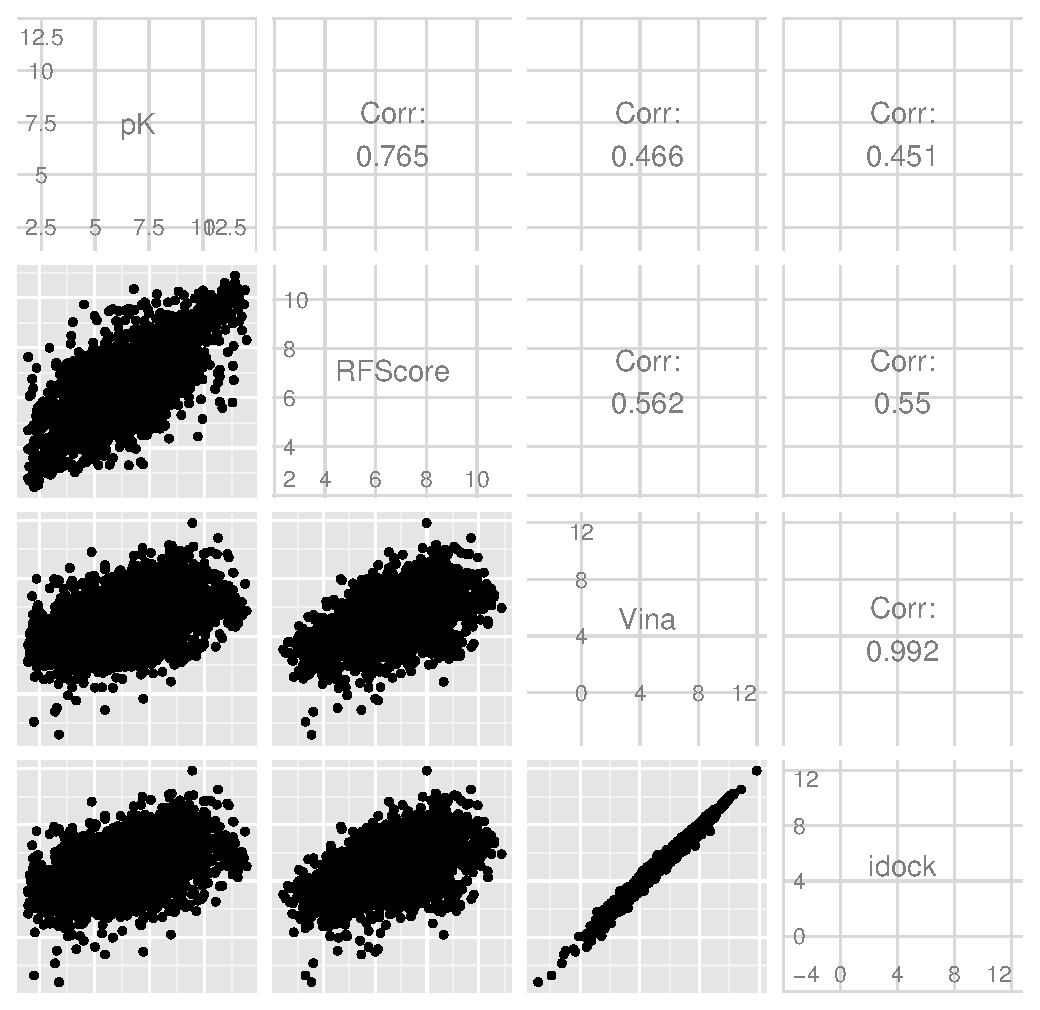
\includegraphics[width=\linewidth]{../istar/PDBbind2012Correlations.eps}
\end{center}
\caption{Correlations between experimental and predicted binding affinity on PDBbind v2012 refined set.}
\label{istar:PDBbind2012Correlations}
\end{figure}

\begin{figure}
\begin{center}
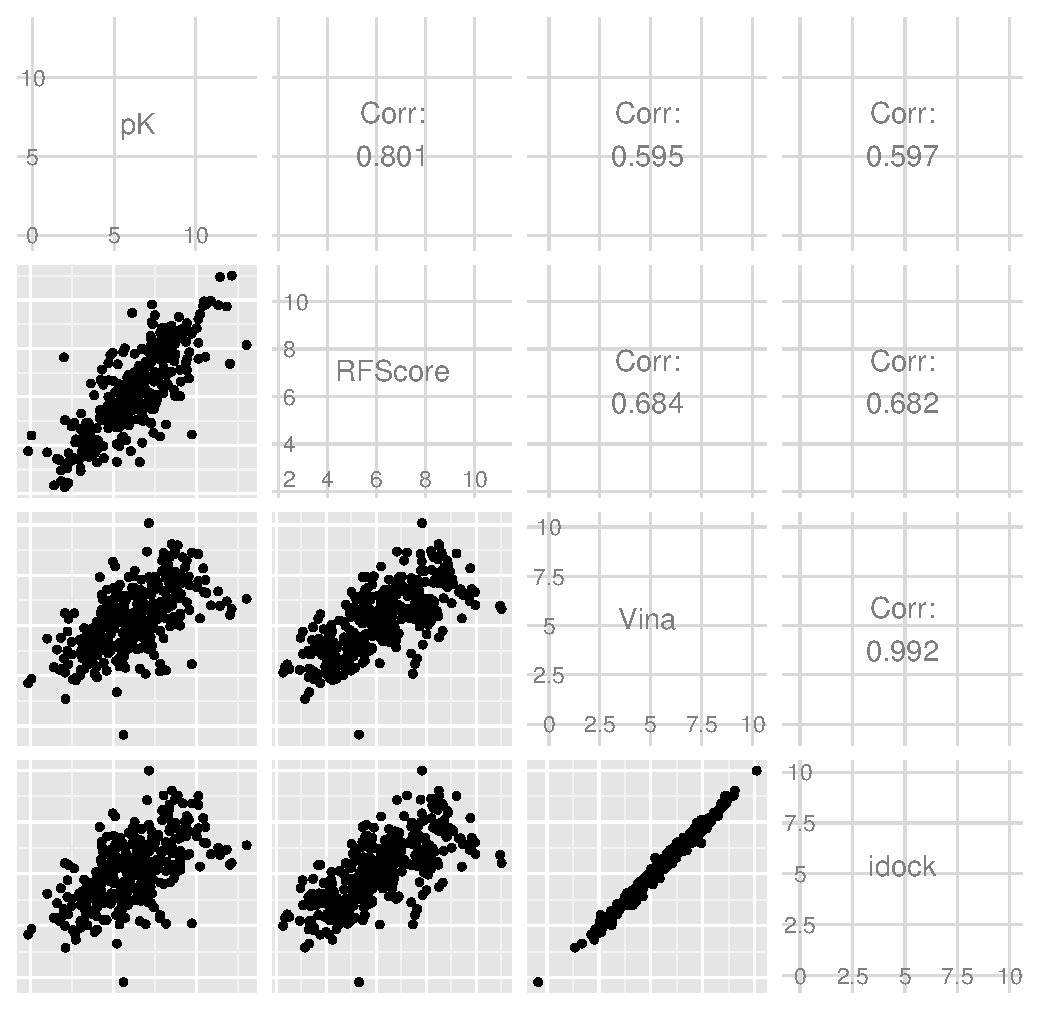
\includegraphics[width=\linewidth]{../istar/CSAR2010Correlations.eps}
\end{center}
\caption{Correlations between experimental and predicted binding affinity on CSAR NRC HiQ Set 24Sept2010.}
\label{istar:CSAR2010Correlations}
\end{figure}

\subsection{Redocking results}

Figure \ref{istar:RedockingVisualization} visualizes the redocking results of four protein-ligand complexes selected from the PDBbind v2012 refined set. The crystal ligand conformation is rendered in green. The conformation predicted by Vina is rendered in red. The conformation predicted by idock is rendered in blue. In (a), the protein target is purine nucleoside phosphorylase. $RMSD$ = 0.14\AA\ for Vina, and $RMSD$ = 0.13\AA\ for idock. Both methods managed to predict a conformation sufficiently close to that of the co-crystallized ligand. In (b), the protein target is thermolysin. $RMSD$ = 8.40\AA\ for Vina, and $RMSD$ = 9.91\AA\ for idock. Both methods failed to predict a conformation sufficiently close to that of the co-crystallized ligand, probably due to the presence of a zinc ion in the binding site. In (c), the protein target is bifunctional purine biosynthesis protein PURH. $RMSD$ = 7.06\AA\ for Vina, and $RMSD$ = 0.21\AA\ for idock. idock managed to predict a conformation sufficiently close to that of the co-crystallized ligand but AutoDock Vina failed. In (d), the protein target is FimX. $RMSD$ = 0.29\AA\ for Vina, and $RMSD$ = 10.23\AA\ for idock. AutoDock Vina managed to predict a conformation sufficiently close to that of the co-crystallized ligand but idock failed.

\begin{figure}
\centering
\subfloat[PDB 1B8N.]
{
  \includegraphics[width=0.48\linewidth]{../istar/Redocking1B8N.png}
}
\subfloat[PDB 4TMN.]
{
  \includegraphics[width=0.48\linewidth]{../istar/Redocking4TMN.png}
}
\\
\subfloat[PDB 1PKX.]
{
  \includegraphics[width=0.48\linewidth]{../istar/Redocking1PKX.png}
}
\subfloat[PDB 3HV8.]
{
  \includegraphics[width=0.48\linewidth]{../istar/Redocking3HV8.png}
}
\caption{Redocking visualization of four protein-ligand complexes.}
\label{istar:RedockingVisualization}
\end{figure}

Table \ref{istar:RedockingSuccessRate} shows the success rates of idock and AutoDock Vina on the PDBbind v2012 refined set ($N$ = 2,897), the PDBbind v2011 refined set ($N$ = 2,455), and the CSAR NRC HiQ Set 24Sept2010 ($N$ = 343) under various conditions regarding the $RMSD$ values between the crystal and docked conformations. By default, both programs output 9 predicted conformations per ligand. Given a redocking case, $RMSD_i (i = 1,2,...,9)$ refers to the $RMSD$ value between the crystal conformation and the $i$th docked conformation, i.e. the one with the $i$th highest predicted binding affinity, whereas $RMSD_{min}$ refers to the $RMSD$ value between the crystal conformation and the closest docked conformation, i.e. the one with the minimum $RMSD$ value. $RMSD_{min} = \displaystyle\min_{i\in[1, 9]}RMSD_i$. The condition $RMSD_1$ = $RMSD_{min}$ therefore tests for how many percent the docked conformation with the highest predicted binding affinity actually turns out to be the closest one among the 9 predicted conformations to the crystal conformation. It can be seen that the success rates of idock are comparable to, albeit slightly lower than, AutoDock Vina, and the success rates on the CSAR NRC HiQ Set 24Sept2010 are consistently higher than the PDBbind v2012 and v2011 refined sets, probably because the scoring function performs well on carefully refined structures. Using a $RMSD$ value of 2.0\AA, a publicly accepted positive control for correct bound structure prediction, both programs managed to predict a conformation sufficiently close to that of the co-crystallized ligand as the first conformation in over half of the cases, without any manual tweaking of the protein model.

\begin{table}
\caption{Redocking success rates of idock and AutoDock Vina.}
\label{istar:RedockingSuccessRate}
\begin{tabular}{lrrrrrr}
\hline
& \multicolumn{2}{c}{PDBbind v2012} & \multicolumn{2}{c}{PDBbind v2011} & \multicolumn{2}{c}{CSAR NRC HiQ}\\
Condition & idock & Vina & idock & Vina & idock & Vina\\
\hline
$RMSD_1$ = $RMSD_{min}$         & 49\% & 53\% & 47\% & 54\% & 59\% & 71\%\\
$RMSD_2$ = $RMSD_{min}$         & 15\% & 16\% & 16\% & 14\% & 18\% & 13\%\\
$RMSD_3$ = $RMSD_{min}$         &  8\% &  7\% &  8\% &  8\% &  4\% &  4\%\\
$RMSD_4$ = $RMSD_{min}$         &  6\% &  6\% &  6\% &  5\% &  7\% &  3\%\\
$RMSD_5$ = $RMSD_{min}$         &  5\% &  4\% &  5\% &  5\% &  3\% &  1\%\\
$RMSD_6$ = $RMSD_{min}$         &  5\% &  3\% &  5\% &  4\% &  3\% &  3\%\\
$RMSD_7$ = $RMSD_{min}$         &  4\% &  4\% &  5\% &  4\% &  2\% &  2\%\\
$RMSD_8$ = $RMSD_{min}$         &  5\% &  3\% &  4\% &  3\% &  3\% &  2\%\\
$RMSD_9$ = $RMSD_{min}$         &  4\% &  3\% &  4\% &  3\% &  1\% &  2\%\\
\noalign{\smallskip}
$RMSD_1$     \textless\ 0.5 \AA & 10\% & 12\% & 11\% & 12\% & 20\% & 21\%\\
$RMSD_1$     \textless\ 1.0 \AA & 26\% & 31\% & 29\% & 31\% & 45\% & 47\%\\
$RMSD_1$     \textless\ 1.5 \AA & 43\% & 47\% & 45\% & 47\% & 61\% & 67\%\\
$RMSD_1$     \textless\ 2.0 \AA & 51\% & 56\% & 53\% & 56\% & 70\% & 73\%\\
$RMSD_1$     \textless\ 2.5 \AA & 56\% & 61\% & 58\% & 61\% & 73\% & 76\%\\
\noalign{\smallskip}
$RMSD_{min}$ \textless\ 0.5 \AA & 12\% & 14\% & 14\% & 15\% & 27\% & 26\%\\
$RMSD_{min}$ \textless\ 1.0 \AA & 35\% & 40\% & 39\% & 40\% & 60\% & 55\%\\
$RMSD_{min}$ \textless\ 1.5 \AA & 61\% & 65\% & 64\% & 65\% & 82\% & 84\%\\
$RMSD_{min}$ \textless\ 2.0 \AA & 72\% & 79\% & 74\% & 78\% & 88\% & 92\%\\
$RMSD_{min}$ \textless\ 2.5 \AA & 77\% & 85\% & 79\% & 84\% & 91\% & 94\%\\
\hline
\end{tabular}
\end{table}

We attempted to examine two possible reasons that might cause idock to fail in some redocking test cases. They are the number of rotatable bonds of the ligand and the number of metal ions in the binding site. Figure \ref{istar:Program-NRB} plots the impact of rotatable bonds of the ligand on the redocking success rates of idock and AutoDock Vina benchmarked on PDBbind v2012 core set ($N$ = 201). Out of the 201 cases, there are 109 and 114 successful cases for idock and AutoDock Vina respectively. The average number of rotatable bonds of the ligand in successful cases are 7.52 and 7.30 respectively for idock and AutoDock Vina. The average number of rotatable bonds of the ligand in unsuccessful cases are 10.36 and 10.82 respectively for idock and AutoDock Vina. Both programs tended to do well when the ligand contains fewer than 10 rotatable bonds.

\begin{figure}
\begin{center}
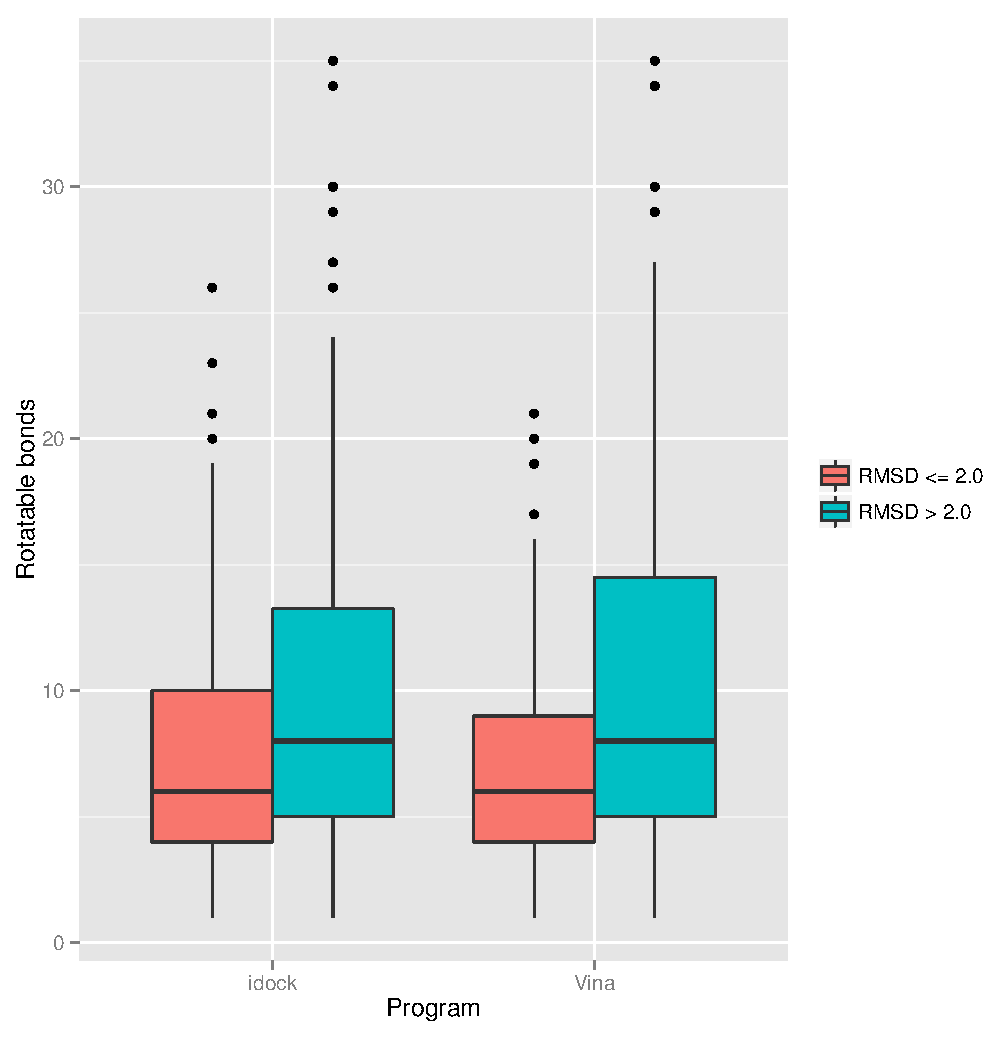
\includegraphics[width=\linewidth]{../istar/Program-NRB.eps}
\end{center}
\caption{Impact of rotatable bonds of the ligand on redocking success rates.}
\label{istar:Program-NRB}
\end{figure}

Figure \ref{istar:Program-NIONS} plots the impact of metal ions in the binding site on the redocking success rates of idock and AutoDock Vina benchmarked on PDBbind v2012 core set ($N$ = 201). Out of the 201 cases, there are 158, 31 and 12 cases in which there are 0, 1 and 2 metal ions respectively in the binding site. For idock, the success rates are 0.58, 0.39 and 0.42 when there are 0, 1 and 2 metal ions respectively in the binding site. For AutoDock Vina, they are 0.60, 0.42 and 0.50 respectively. Both programs tended to do well when the binding site contains no metal ions.

\begin{figure}
\begin{center}
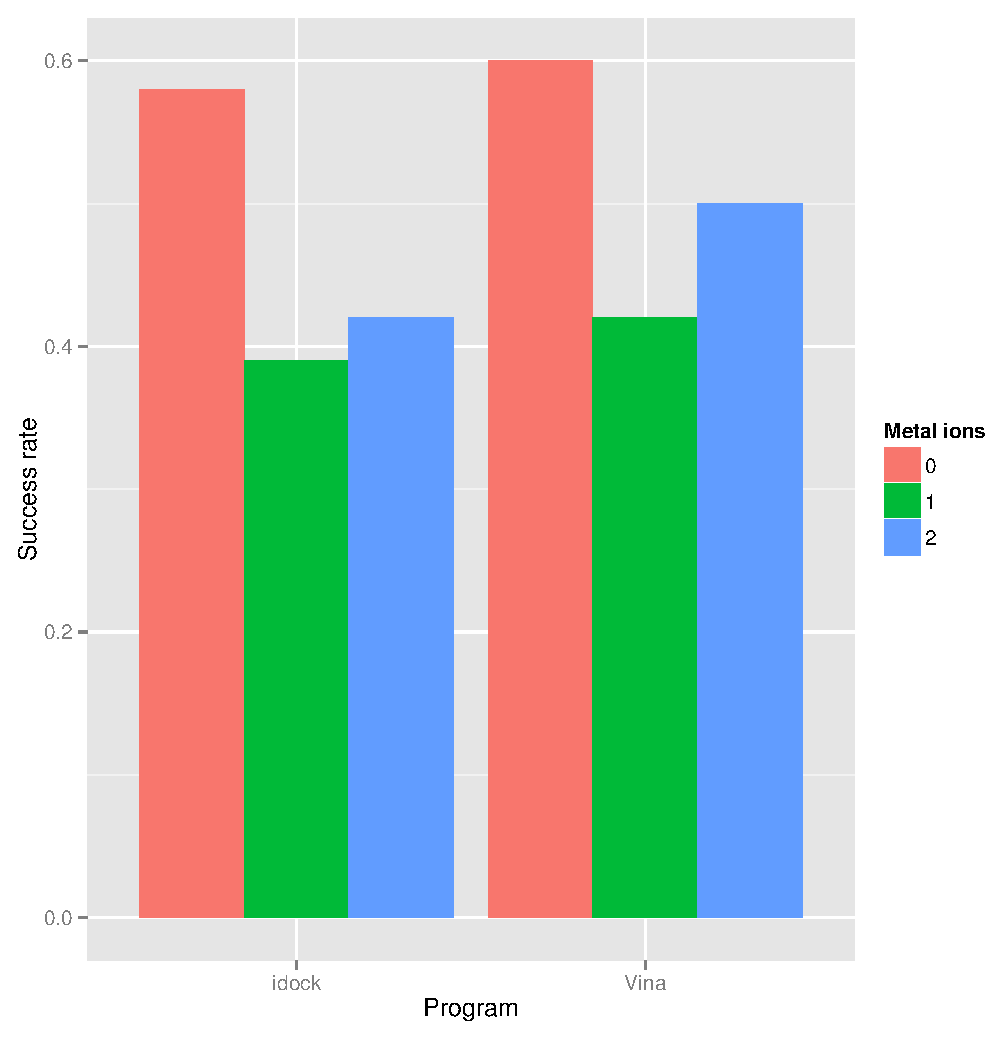
\includegraphics[width=\linewidth]{../istar/Program-NIONS.eps}
\end{center}
\caption{Impact of metal ions in the binding site on redocking success rates.}
\label{istar:Program-NIONS}
\end{figure}

Figure \ref{istar:VinaConf1RMSD-idockConf1RMSD} shows the $RMSD_1$ values for idock plotted against those for AutoDock Vina. The color encodes the number of rotatable bonds (NRB) of the ligand. Many points fall onto the diagonal, suggesting that both programs tended to predict similar conformations.

\begin{figure}
\begin{center}
\includegraphics[width=\linewidth]{../istar/VinaConf1RMSD-idockConf1RMSD.eps}
\end{center}
\caption{$RMSD_1$ of the predicted ligand conformation.}
\label{istar:VinaConf1RMSD-idockConf1RMSD}
\end{figure}

From the perspective of prospective docking, Figure \ref{istar:pK-idockConf1idock} shows the scatter plot of the highest predicted binding affinity of the 9 docked conformations output by idock against the experimental binding affinity on PDBbind v2012 core set ($N$ = 201) in the redocking benchmark. Values are in $pK_d$ or $pK_i$ unit. The weak correlation and large deviation ($R_p$ = 0.502, $R_s$ = 0.530, $RMSE$ = 1.31, $SD$ = 1.32) reflect the limitation of using idock alone as scoring function. After re-training RF-Score on PDBbind v2012 refined set ($N$ = 2,897) and adopting the maximum RF-Score of the 9 docked conformations as predicted binding affinity, the correlation was improved (Figure \ref{istar:pK-idockConfsRFScoreMax}, $R_p$ = 0.815, $R_s$ = 0.817, $RMSE$ = 0.75, $SD$ = 0.76). Moreover, since for over 50\% probability the docked conformation with the highest predicted binding affinity indeed turned out to be the closest to the crystal conformation (i.e. $RMSD_1$ = $RMSD_{min}$), using RF-Score to re-score the conformation with $RMSD_1$ led to even better prediction (Figure \ref{istar:pK-idockConf1RFScore}, $R_p$ = 0.855, $R_s$ = 0.859, $RMSE$ = 0.73, $SD$ = 0.73).

\begin{figure}
\begin{center}
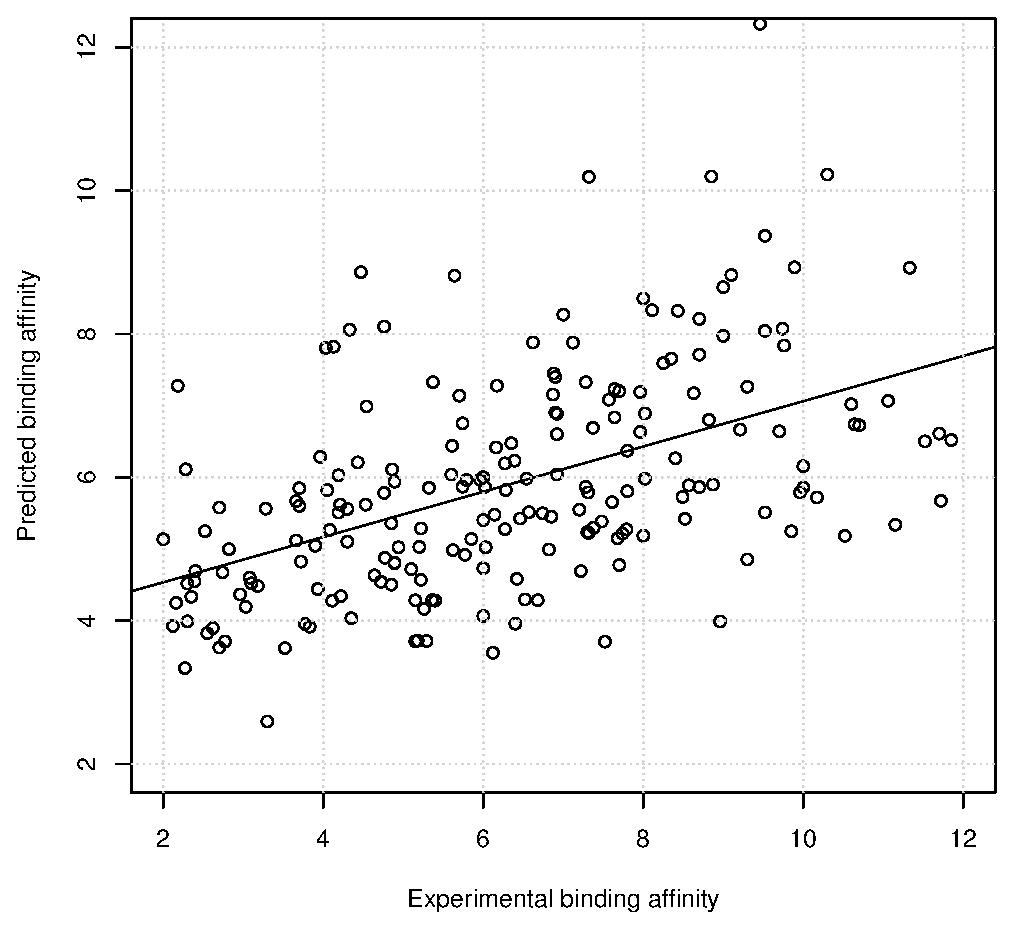
\includegraphics[width=\linewidth]{../istar/pK-idockConf1idock.eps}
\end{center}
\caption{Scatter plot of the lowest idock score of the 9 docked conformations against the experimental binding affinity.}
\label{istar:pK-idockConf1idock}
\end{figure}

\begin{figure}
\begin{center}
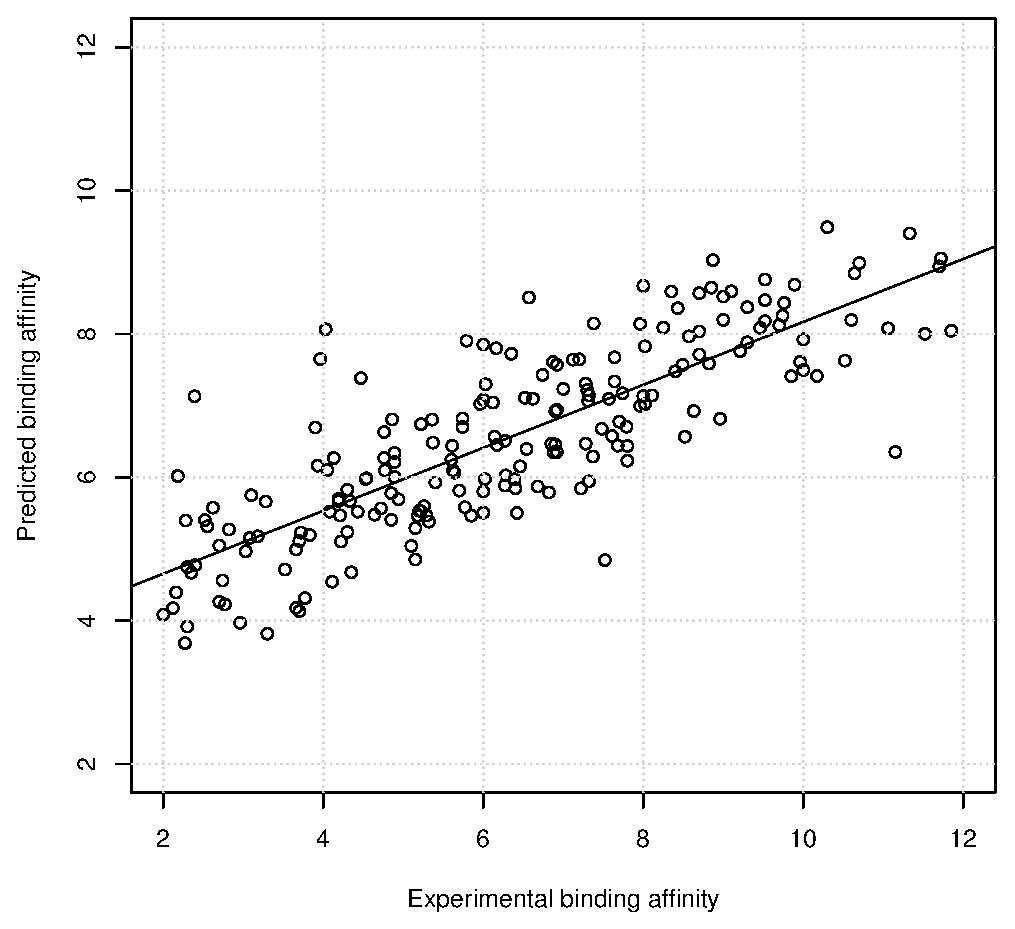
\includegraphics[width=\linewidth]{../istar/pK-idockConfsRFScoreMax.eps}
\end{center}
\caption{Scatter plot of the highest RF-Score of the 9 docked conformations against the experimental binding affinity.}
\label{istar:pK-idockConfsRFScoreMax}
\end{figure}

\begin{figure}
\begin{center}
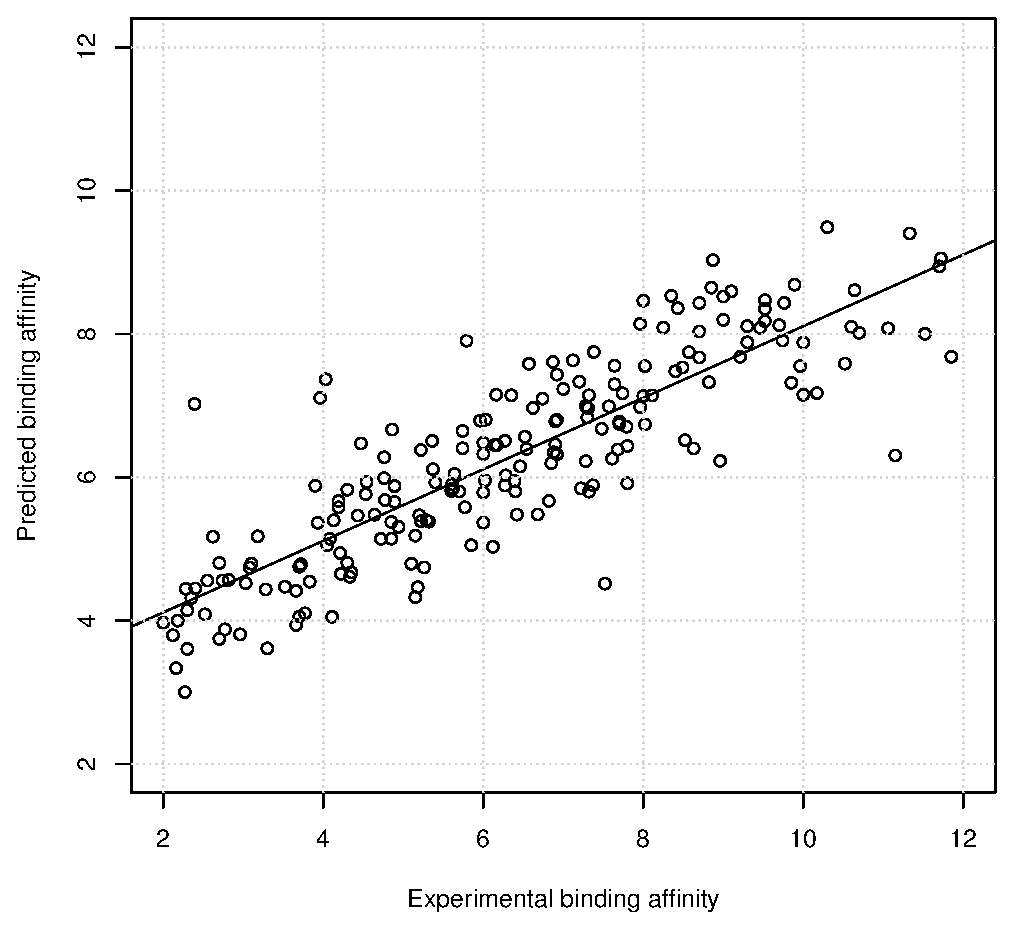
\includegraphics[width=\linewidth]{../istar/pK-idockConf1RFScore.eps}
\end{center}
\caption{Scatter plot of the RF-Score of the first docked conformation against the experimental binding affinity.}
\label{istar:pK-idockConf1RFScore}
\end{figure}

\subsection{Execution time results}

Table \ref{istar:ExecutionTime} compares the CPU time and elapsed time in hours of docking 3,000 clean ligands in 3 molecular weight sets against 12 diverse receptors by AutoDock Vina and idock. As expected, the execution time varied considerably from protein to protein and from molecular weight set to molecular weight set. Overall, idock outperformed AutoDock Vina by at least 8.69 times and at most 37.51 times, making idock particularly ideal for large-scale docking, as is the case of istar.

\begin{table}
\caption{Execution time of AutoDock Vina and idock.}
\label{istar:ExecutionTime}
\begin{tabular}{lrrrrrr}
\hline
& \multicolumn{2}{c}{200-300g/mol} & \multicolumn{2}{c}{300-400g/mol} & \multicolumn{2}{c}{400-500g/mol}\\
& CPU & Elapsed & CPU & Elapsed & CPU & Elapsed\\
\hline
\multicolumn{7}{l}{\textbf{1HCL} human cyclin-dependent kinase 2}\\
Vina  & 12.57 &  3.33 & 22.55 &  5.91 & 51.62 & 13.41\\
idock &  0.63 &  0.16 &  0.92 &  0.24 &  1.38 &  0.36\\
\multicolumn{7}{l}{\textbf{1J1B} human tau protein kinase I}\\
Vina  &  9.07 &  2.47 & 14.69 &  3.92 & 32.28 &  8.49\\
idock &  0.78 &  0.21 &  1.25 &  0.33 &  2.35 &  0.62\\
\multicolumn{7}{l}{\textbf{1LI4} human S-adenosylhomocysteine hydrolase}\\
Vina  & 11.82 &  3.30 & 19.08 &  5.22 & 39.41 & 10.64\\
idock &  0.89 &  0.23 &  1.55 &  0.40 &  3.15 &  0.82\\
\multicolumn{7}{l}{\textbf{1V9U} human rhinovirus 2 coat protein VP1}\\
Vina  &  9.80 &  2.95 & 15.55 &  4.62 & 29.75 &  8.49\\
idock &  0.97 &  0.25 &  1.64 &  0.42 &  3.42 &  0.89\\
\multicolumn{7}{l}{\textbf{2IQH} influenza A virus nucleoprotein NP}\\
Vina  &  9.51 &  2.66 & 15.03 &  4.08 & 29.64 &  7.83\\
idock &  0.92 &  0.24 &  1.59 &  0.41 &  3.41 &  0.88\\
\multicolumn{7}{l}{\textbf{2XSK} Escherichia coli curli protein CsgC - SeCys}\\
Vina  & 10.44 &  2.71 & 17.89 &  4.61 & 40.58 & 10.41\\
idock &  0.71 &  0.19 &  1.16 &  0.30 &  2.16 &  0.56\\
\multicolumn{7}{l}{\textbf{2ZD1} HIV-1 reverse transcriptase}\\
Vina  &  9.78 &  2.70 & 17.67 &  4.76 & 42.03 & 11.33\\
idock &  0.97 &  0.25 &  1.52 &  0.39 &  2.60 &  0.69\\
\multicolumn{7}{l}{\textbf{2ZNL} influenza virus RNA polymerase subunit PA}\\
Vina  &  9.49 &  2.60 & 15.04 &  4.01 & 29.97 &  7.82\\
idock &  0.89 &  0.23 &  1.56 &  0.40 &  3.41 &  0.87\\
\multicolumn{7}{l}{\textbf{3BGS} human purine nucleoside phosphorylase}\\
Vina  &  9.59 &  2.57 & 16.50 &  4.37 & 38.42 & 10.14\\
idock &  0.95 &  0.25 &  1.55 &  0.40 &  2.81 &  0.74\\
\multicolumn{7}{l}{\textbf{3H0W} human S-adenosylmethionine decarboxylase}\\
Vina  &  9.85 &  2.64 & 17.67 &  4.70 & 41.69 & 11.04\\
idock &  0.88 &  0.23 &  1.35 &  0.35 &  2.20 &  0.58\\
\multicolumn{7}{l}{\textbf{3IAR} human adenosine deaminase}\\
Vina  & 11.25 &  3.03 & 20.21 &  5.39 & 46.93 & 12.53\\
idock &  0.80 &  0.21 &  1.21 &  0.32 &  2.01 &  0.53\\
\multicolumn{7}{l}{\textbf{3KFN} HIV protease}\\
Vina  & 10.53 &  2.80 & 18.37 &  4.83 & 42.43 & 11.03\\
idock &  0.77 &  0.20 &  1.20 &  0.32 &  2.09 &  0.55\\
\multicolumn{7}{l}{\textbf{Average across the above 12 receptors}}\\
Vina  & 10.31 &  2.81 & 17.52 &  4.70 & 38.73 & 10.26\\
idock &  0.85 &  0.22 &  1.38 &  0.36 &  2.58 &  0.67\\
\hline
\end{tabular}
\end{table}

\section{Discussion}

Docking is a computational method that investigates how a ligand binds to a protein, and predicts their binding affinity. Hence docking is useful in elaborating inter-molecular interactions and enhancing the potency and selectivity of binding in subsequent phases of the drug discovery process.

In this study, we report a web platform called istar to automate large-scale protein-ligand docking using our popular docking engine idock. Since the initial release of idock, we have been further improving its docking speed and robustness. Compared to AutoDock Vina, our idock features a new numerical model in approximation of the scoring function, replacing slow linear interpolation by fast table lookup. It encapsulates a unique feature that can safely deactivate certain torsions to reduce the dimension of variables. It also implements an efficient thread pool to parallelize multiple components of the program and maintain a high CPU utilization. Results show that idock managed to predict a conformation sufficiently close to that of the co-crystallized ligand as the first conformation in over half of the test cases across a number of diverse datasets, and it outperformed AutoDock Vina by an order of magnitude in terms of docking efficiency at no significant cost of accuracy. It is worthwhile to highlight that in order to use istar, the input protein model requires no manual preprocessing in most cases.

We examined two possible reasons that might cause idock to fail in some test cases. They are the number of rotatable bonds of the ligand and the number of metal ions in the binding site. On one hand, a large number of rotatable bonds implies a high dimension of variables to optimize. idock has a higher chance to succeed when the ligand consists of fewer than 10 rotatable bonds. On the other hand, all kinds of metal ions are treated as hydrogen bond donors in the idock scoring function, which might not thoroughly account for their solvation effects and other possible interactions. idock has a higher chance to succeed when the binding site consists of no metal ions.

Although idock performs well in conformation prediction, it displays weakness in binding affinity prediction. In contrast, RF-Score, a new scoring function that circumvents the need for problematic modelling assumptions via non-parametric machine learning, has been recently shown to obtain the best scoring performance among 16 classical scoring functions on PDBbind v2007 core set ($N$ = 195) \citep{564}. We have therefore integrated a revised version of RF-Score as an alternative re-scoring function. We have re-trained RF-Score on the entire PDBbind v2012 refined set ($N$ = 2,897) for prospective prediction purpose. Results show that using RF-Score to re-score the predicted conformations led to a much better prediction with $R_p$ = 0.855, $R_s$ = 0.859, $RMSE$ = 0.73, and $SD$ = 0.73. We have successfully demonstrated that RF-Score is a particularly effective re-scoring function for docking purposes.

To compile a more complete list of scoring functions benchmarked on the PDBbind v2007 core set ($N$ = 195) into Table \ref{istar:ScoringFunctionComparison}, we have extracted the performance results for 19 scoring functions from \citep{1313,564,1305,1295}, and reported the results for AutoDock Vina and idock on the same test set in this study. This procedure has a number of advantages. Evaluating all the scoring functions on the same test set under the same conditions guarantees a fair and objective comparison. Using a common existing benchmark can also ensure the optimal application of such functions by their authors and avoid the danger of constructing an in-house benchmark on which unrealistically high performance might be produced. Moreover, future scoring functions can be unambiguously incorporated into this comparative assessment. Notably, the top four scoring functions, namely RF-Score \citep{564}, ID-Score \citep{1305}, SVR-Score \citep{1295} and X-Score \citep{573}, are the only scoring functions whose training set do not overlap with the PDBbind v2007 core set. The prediction power of RF-Score is already superior to many scoring functions employed in commercial docking software. In terms of implementation complexity, a descriptor in RF-Score is just the occurrence count of a particular protein-ligand atom type pair interacting within a certain distance range, while a descriptor in ID-Score can be as mathematically demanding as, for instance, calculating the cosine value of the bond angle between a hydrogen bond donor and a hydrogen bond acceptor. This again demonstrates the adaptiveness of RF-Score to various applications.

One may argue that although the scoring functions are evaluated on the same test set, their training sets are not identical. Besides, the PDBbind v2007 core set consists of merely 195 complexes, which might not cover sufficient protein-ligand diversity from the perspective nowadays. To address this issue, we re-trained RF-Score on the PDBbind v2007 refined set ($N$ = 1,300), on which AutoDock Vina and idock were also trained, and we expanded the test set to the much larger PDBbind v2012 refined set ($N$ = 2,897). Figure \ref{istar:PDBbind2012Correlations} clearly shows that all the performance gain ($R_p$ = 0.765, $R_s$ = 0.755, $RMSE$ = 1.26, $SD$ = 1.26 for RF-Score versus $R_p$ = 0.451, $R_s$ = 0.453, $RMSE$ = 1.75, $SD$ = 1.75 for idock) is guaranteed to come from the scoring function characteristics, ruling out any influence of using different training sets on performance.

In computational biology, ten simple rules have been summarized for providing a scientific web resource \citep{677}. Software and web sites do count for getting ahead as a computational biologist \citep{260}. To design the istar platform in a user-friendly way, we have utilized state-of-the-art web and database technologies. On istar, there are over 23 million ready-to-dock ligands collected from ZINC \citep{532,1178}. These ligands come with supplier information for easy purchasing, and they can be filtered by nine molecular properties in a fine-grained manner. The number of ligands to dock can be previewed in real time. The jobs are transparently split into slices for parallel docking across multiple workstations, and the job progress can be monitored in real time in a browser so that users can have a rough estimation of how long the job will take and when the job will complete. Additionally, our web server supports REST API, by programming against which users can submit multiple jobs in batch. Automation is the major reason of submitting jobs to istar instead of running idock locally on one's computer. With istar at hand, users need not to write special scripts to fetch ligands from some sources, to implement parallelism, or to invoke RF-Score externally by themselves. Users can therefore concentrate on the docking results and subsequent analysis rather than the docking process itself.

We compare our istar to DOCK Blaster \citep{557}, an expert system created to investigate the feasibility of full automation of large-scale protein-ligand docking. It uses DOCK 3 \citep{1445} as the docking engine and ZINC \citep{532,1178} as the ligand repository. Although DOCK is open source, DOCK Blaster itself is closed source. istar is indeed much easier to use than DOCK Blaster. Given the structure of a target protein, both istar and DOCK Blaster can dock and score a large set of ligands against the target protein and provide a ranked list which users may review and prioritize for purchasing and wet-lab testing. From the perspective of binding site indication, istar automatically detects a site from the co-crystallized ligand, while DOCK Blaster uses PocketPickker (CLIPPERS) \citep{395}. From the perspective of ligand selection, istar features ligand filtering by nine desired molecular properties in a fine-grained fashion, while DOCK Blaster predefines several subsets either by property, by vendor, or by user. From the perspective of documentation and user manual, the istar website presents a series of graphical tutorials on how to submit a new job and other related issues, while DOCK Blaster deploys a wiki with very rich contents covering all the relevant procedures. As extra features, DOCK Blaster allows the input of known active and inactive binders as heuristic information for docking. In summary, although istar and DOCK Blaster share the identical motivation of automating large-scale protein-ligand docking, their internal implementations and methodologies differ greatly. Users are encouraged to utilize both istar and DOCK Blaster as well as other docking servers to reach a consensus of promising candidate ligands.

According to Google Analytics, throughout September 2014, istar had 647 sessions, 334 users, and 1848 pageviews from 43 countries. According to our internal statistics, from October 2013 to October 2014, there had been 635 job submissions with 46,581,105 ligands docked. These jobs came from 126 email addresses, 64 of which were associated with multiple jobs while the other 62 were associated with one single job. Due to limited budget, we cannot offer as much hardware resource as DOCK Blaster (i.e. 700 CPU cores plus 20TB RAID-6 storage). However, we emphasize full reproducibility \citep{965} and we have released istar under a permissive open source license so that anyone who possesses sufficient hardware resource is welcome to deploy a copy of istar to his/her own infrastructure with no charge. On a related issue, we can draw on the experience of QMachine \citep{1405}, an open-sourced, publicly available web service that acts as a messaging system for posting tasks and retrieving results over HTTP in a PaaS (Platform as a Service) manner. It aggregates commodity hardware and volunteer compute cycles to enable commodity supercomputing in web browsers. Few server resources are required because all analytical and data retrieval tasks are executed by volunteer machines.

\section{Conclusions}

In this study we report istar \citep{1362}, our SaaS platform for bioinformatics and chemoinformatics applications, with idock \citep{1153} being a particular instance of large-scale online protein-ligand docking. We believe the huge body of existing AutoDock users can easily transit to the idock service on istar, which we believe constitutes a step toward generalizing the use of docking tools beyond the traditional molecular modeling community.

As a versatile web platform, istar also aggregates our other software and provides them as services. These include a pragmatic implementation of USR (Ultrafast Shape Recognition) \citep{1379} and USRCAT (USR with Credo Atom Types) \citep{1331} for prospective ligand-based virtual screening, iview \citep{1366} for interactive WebGL visualization of protein-ligand complex, igrep \citep{1138} for approximate DNA/RNA sequence matching, and icuda as an introductory seminar series about CUDA programming. We encourage our colleagues to host their software as services on istar so that more users can benefit.

\section{Availability}

istar is free and open source under Apache License 2.0. Its C++ and JavaScript source code is available at https://github.com/HongjianLi/istar. Our deployment of istar is running at http://istar.cse.cuhk.edu.hk/.

\section{Acknowledgements}

We thank Professor John J. Irwin for granting us permission to use ZINC \citep{532,1178} with three conditions:
\begin{enumerate}
\item We shall provide links to http://zinc.docking.org/substance/zincid for top hits so that users can seek for the most current purchasing information at ZINC's official website.
\item We shall limit the number of top hits for download to 1000 ligands from a single job.
\item We shall update our ligands when ZINC data is updated so that users can benefit from the most current ligand data.
\end{enumerate}

\section{Future works}

idock has been evaluated from the perspectives of rescoring, redocking, and execution time, but it has not been evaluated from the perspective of enrichment, which requires the active ligands be ranked high in a set of decoys. In this case BEDROC \citep{490} and SLR \citep{489} could be used as performance measures for the ``early recognition" problem.

\chapterend
